\documentclass[12pt,reqno]{article}

\usepackage[usenames]{color}
\usepackage{amssymb}
\usepackage{amsmath}
\usepackage{amsthm}
\usepackage{amsfonts}
\usepackage{amscd}
\usepackage{graphicx}
\usepackage{xcolor}
\usepackage{float}
\usepackage{booktabs}
\usepackage[margin=.8in]{geometry}
\usepackage{amsmath,amssymb,mathtools}
\usepackage{booktabs}
\usepackage{microtype}
\usepackage{tikz}
\usepackage[colorlinks=true,linkcolor=blue,citecolor=blue,urlcolor=blue]{hyperref}

\def\modd#1 #2{#1\ \mbox{\rm (mod}\ #2\mbox{\rm )}}

\usepackage[colorlinks=true,
linkcolor=webgreen,
filecolor=webbrown,
citecolor=webgreen]{hyperref}

\definecolor{webgreen}{rgb}{0,.5,0}
\definecolor{webbrown}{rgb}{.6,0,0}


\usepackage{fullpage}

%\usepackage{psfig}
\usepackage{graphics}
\usepackage{latexsym}
\usepackage{epsf}
\usepackage{breakurl}

\setlength{\textwidth}{6.5in}
\setlength{\oddsidemargin}{.1in}
\setlength{\evensidemargin}{.1in}
\setlength{\topmargin}{-.1in}
\setlength{\textheight}{8.4in}

\newcommand{\seqnum}[1]{\href{https://oeis.org/#1}{\rm \underline{#1}}}

\newcommand{\Z}{\mathbb Z}
\newcommand{\N}{\mathbb N}
\newcommand{\word}[1]{\mathtt{#1}}
\newcommand{\vp}{\nu_3}
\newcommand{\vTwo}{\nu_2}

\newcommand{\Q}{\mathbb{Q}}
\newcommand{\wt}{\mathbf{t}}
\newcommand{\ws}{\mathbf{s}}
\newcommand{\ww}{\mathbf{w}}

\DeclareMathOperator{\Par}{\psi}

\begin{document}


\theoremstyle{plain}
\newtheorem{theorem}{Theorem}
\newtheorem{corollary}[theorem]{Corollary}
\newtheorem{lemma}[theorem]{Lemma}
\newtheorem{proposition}[theorem]{Proposition}

\theoremstyle{definition}
\newtheorem{definition}[theorem]{Definition}
\newtheorem{example}[theorem]{Example}
\newtheorem{conjecture}[theorem]{Conjecture}

\theoremstyle{remark}
\newtheorem{remark}[theorem]{Remark}

\author{Stijn Cambie \and E. Kalviainen \and J. Shallit\\
School of Computer Science\\
University of Waterloo\\
Waterloo, ON  N2L 3G1 \\
Canada\\
\href{mailto:shallit@uwaterloo.ca}{\tt shallit@uwaterloo.ca}}

\title{Brown-Gerver-Ramsey Theorems in Small Dimensions}

\maketitle

\begin{abstract}
We consider infinite walks in $\N^k$ with standard unit basis vector steps that avoid
$t$ collinear points, and show these walks exist for $(k,t) \in \{(6,3), (4,4), (3,7)\}$.  In particular, our construction for $k = 3$ improve the previous bound $189$, obtained by Lidbetter, to $7$.  Our results also imply construction of infinite words over small finite alphabets that are weakly abelian squarefree (resp., weakly abelian cubefree, weakly abelian 6th-power-free).
\end{abstract}

\section{Introduction}

In 1971 Tom C. Brown observed that every infinite walk on the lattice points of the plane, using only the steps $(0,1)$ and $(1,0)$, must contain $n$ collinear points for all $n \geq 2$.  He submitted his result to the Advanced Problem section of the {\it American Mathematical Monthly} \cite{Bro71b}, and a nice solution was published in 1972 by Peter Montgomery \cite{Mo72}.

(Of course, it is easy to create such a walk without {\it infinitely many\/} collinear points:  for example, set $P_0 = (0,0)$, and
$$ P_{n+1} = \begin{cases}
    P_n + (0,1), & \text{if $P_n = (k^2,k-1)$ for some integer $k$}; \\
    P_n + (1,0), & \text{otherwise.} 
    \end{cases}
$$
The resulting walk resembles a parabola and every line intersects the walk at only finitely many points.)

Brown's observation was generalized by Gerver and Ramsey to the case where the steps are chosen from an arbitrary fixed finite set $S \subseteq \N^2$ \cite{GR79}.
Gerver and Ramsey also found an upper bound on the walk length guaranteeing the existence of $n$ collinear points, as a function of the size of $S$ and the norm of the largest step.

Gerver and Ramsey addressed the same question in $\N^3$.  For that version of the problem, they proved there is an infinite walk, using only the
unit vector steps 
$(1,0,0), (0,1,0), (0,0,1)$, with no
$5^{11} + 1 = 48828126$ collinear points.
(This number was recently reduced to 189
by Finn Lidbetter \cite{Lid24}.)
And they also raised the question of what dimension $k$ is required to avoid
three collinear points with a finite set of steps.

Recently this latter question was solved by the first two authors \cite{CK26}.  Their preprint proved the existence of an infinite walk in $\N^3$ using a set of 16 steps. 

In this paper we return to the original question of Brown and restrict our attention to walks in $\N^k$ using only the {\it standard unit basis vectors}, that is, those of the form $${\bf e}_{j,i} = (\, \overbrace{0,\ldots 0}^i, 1, 
\overbrace{0,\ldots, 0}^{k-i-1} \,)$$
for $0 \leq i < n$.  The results in \cite{CK26} immediately show that there is an infinite walk in $\N^{16}$, using only the standard unit basis vectors, with no $3$ collinear points.

We now summarize the main results of this paper.  All these walks use only the unit standard basis vectors as steps.

\begin{itemize}
\item Theorem~\ref{thm:main}: there is an infinite walk on $\N^6$
with no $3$ collinear points.  

\item Theorem~\ref{thm:d4}:  there is an infinite walk on $\N^4$ with no $4$ collinear points.

\item Theorem~\ref{thm:d3}:  there is an infinite walk on $\N^3$ with no $7$ collinear points.
\end{itemize}

We do not know if these results can be improved for unit basis vector steps.  For example, we cannot currently rule out an infinite walk on $\N^3$ with
no $4$ collinear points.  We have
constructed a finite walk of length $32768$ with this property.   However, by a result of
Dekking, we know there is no infinite
walk on $\N^3$ with no $3$ collinear points.

We also cannot rule out an infinite walk
in $\N^4$ with no $3$ collinear points.  We have constructed a finite walk of length $5500$ with this property.

Throughout, $\N=\{0,1,2,\ldots\}$, and word and vertex indices start
at zero.

Our constructions use $p$-adic valuations for the primes $p =2$ and $p = 3$.  For a nonzero integer $n$, we let $\nu_p (n)$ be the exponent of the highest power of $p$ dividing $n$. This is extended to nonzero rational numbers $m/n$ by
$\nu_p(m/n) = \nu_p(m) - \nu_p (n)$.

\section{Weak abelian powers}

Our results have a natural interpretation in combinatorics on words.  Let $\Sigma_k = \{0,1,\ldots, k-1\}$ be an alphabet of cardinality $k$.  For a word $w$, let
$|w|_a$ be the number of occurrences of
the letter $a$ in $w$.  For
$w \in \Sigma_k^*$ define
its Parikh vector
$\psi(w)$ to be $(|w|_0, |w|_1, \ldots,
|w|_{k-1})$.
We say that
a word $w$ is a {\it weak abelian $t$'th power} if $w = x_1 x_2 \cdots x_t$, where
each word $x_i$ is nonempty and
$${{\psi(x_1)} \over {|x_1|}} = 
{{\psi(x_1)} \over {|x_2|}} = \cdots =
{{\psi(x_t)} \over {|x_t|}}.$$
We say a word $w$ {\it avoids\/} weak abelian $t$'th powers if no nonempty factor is a weak abelian $t$'th power.  See, for example, \cite{FP23}.

\begin{proposition}
Let $w = w[1..n]$ be a length-$n$ word in $\Sigma_k^*$ 
Consider a walk of length
$n+1$ on $\N^k$ defined by
$P_i(w) = \sum_{1 \leq j \leq i}$ ${\bf e}_{k,j}$ for $0 \leq i \leq n$.  Then
$(P_i(w))_{0 \leq i \leq n}$ has no $t+1$ collinear points iff $w$ has no
weak abelian $t$'th power.
\end{proposition}

\begin{proof}
If there are $t+1$ are collinear points, their
consecutive displacements are positive multiples of a common vector;
division by their coordinate sums gives the same normalized Parikh
vector for all $t$ intervening nonempty blocks. Conversely, such $t$
blocks give $t+1$ collinear boundary vertices.
\end{proof}

Thus our results can be restated as
\begin{itemize}
\item There is an infinite word over $\Sigma_6$
with no weak abelian squares.  

\item There is an infinite word over $\Sigma_4$ with no weak abelian cubes.

\item There is an infinite word over $\Sigma_3$ with no weak abelian $6$th powers.
\end{itemize}


\section{Dimension 6}\label{sec:6}

\begin{theorem}
There is an infinite walk in $\N^6$, using only the standard unit basis vectors as steps, with no $3$ collinear points.
\label{thm:main}
\end{theorem}

We begin with a walk on the Gaussian integers, adapted from the construction in
\cite{CK26}.  Let $i = \sqrt{-1}$, and define $\sigma_n\in\{0,1,2,3\}$ recursively by $\sigma_0=0$ and
\begin{equation}\label{eq:states}
 \sigma_{2n}\equiv \modd{-\sigma_n} {4},
 \qquad
 \sigma_{2n+1}\equiv \modd{1-\sigma_n} {4}.
\end{equation}
For $n \geq 0$, define
\begin{equation}\label{eq:gaussian}
 u_n=i^{\sigma_n},
 \qquad
 z_n=\sum_{0\le r<n}u_r\in\Z[i].
\end{equation}
Thus $(z_n)$ is a nearest-neighbor walk in the Gaussian lattice.  For
$\varepsilon\in\{0,1\}$, Eq.~\eqref{eq:states} gives
\begin{equation}\label{eq:dyadic}
u_{2n+\varepsilon}=i^\varepsilon\,\overline{u_n},
 \qquad
 z_{2n+\varepsilon}
   =(1+i)\, \overline{z_n}+\varepsilon\, \overline{u_n},
\end{equation}
where $\overline{x}$ is the complex conjugate.
Indeed, the second identity follows by pairing
$u_{2r}+u_{2r+1}=(1+i)\overline{u_r}$.

\begin{lemma}\label{lem:chords}
If $0\leq m<n$ and $\sigma_m=\sigma_n$, then $z_m\ne z_n$ and
\begin{equation}\label{eq:chord-valuation}
 \vTwo\bigl(|z_n-z_m|^2\bigr)=\vTwo(n-m).
\end{equation}
\end{lemma}

\begin{proof}
Let $t=\vTwo(n-m)$ and set $(m_0,n_0)=(m,n)$.  We recursively
define pairs $(m_j,n_j)$ for $0\le j\le t$.  Suppose that $j<t$.
Then $n_j-m_j$ is even, so $m_j$ and $n_j$ have the same parity.
Thus, for a unique $\varepsilon_j\in\{0,1\}$, we may write
\[
 m_j=2m_{j+1}+\varepsilon_j,
 \qquad
 n_j=2n_{j+1}+\varepsilon_j.
\]
The two maps
\[
 r\longmapsto-r,\qquad r\longmapsto1-r
\]
are injective on $\mathbb Z/4\mathbb Z$.  Hence the recursion~\eqref{eq:states}, together with
$\sigma_{m_j}=\sigma_{n_j}$, implies
$
 \sigma_{m_{j+1}}=\sigma_{n_{j+1}}
$.
In particular, $u_{m_{j+1}}=u_{n_{j+1}}$.  Applying
\eqref{eq:dyadic} at the two endpoints and subtracting, the correction
terms therefore cancel, giving
\[
 z_{n_j}-z_{m_j}
   =(1+i)\overline{z_{n_{j+1}}-z_{m_{j+1}}}.
\]
Consequently,
\[
 |z_{n_j}-z_{m_j}|^2
   =2|z_{n_{j+1}}-z_{m_{j+1}}|^2.
\]
Iterating for $j=0,\ldots,t-1$ yields
\[
 |z_n-z_m|^2
   =2^t|z_{n_t}-z_{m_t}|^2.
\]

By construction, $n_t-m_t$ is odd.  Moreover,
\[
 z_{n_t}-z_{m_t}
   =\sum_{r=m_t}^{n_t-1}u_r
\]
is a sum of an odd number of elements of $\{1,i,-1,-i\}$.  Write this
sum as $x+iy$.  For each Gaussian unit $u$, the sum of its real and
imaginary coordinates is congruent to $1$ modulo $2$.  Therefore
$x+y$ is odd.  Thus exactly one of $x$ and $y$ is odd, so
\[
 |z_{n_t}-z_{m_t}|^2=x^2+y^2
\]
is odd and, in particular, nonzero.  It follows that $z_n-z_m\ne0$ and
$ \vTwo\bigl(|z_n-z_m|^2\bigr)
   =t
   =\vTwo(n-m)$.
\end{proof}




\begin{proof}[Proof of Theorem~\ref{thm:main}]
Let 
$\delta_n = (\sigma_{n+1}-\sigma_n) \bmod4$.  From~\eqref{eq:states},
\begin{equation}\label{eq:increments}
 \delta_{2n}=1,
 \qquad
 \delta_{2n+1}\equiv-1-\delta_n\pmod4.
\end{equation}
Since $\delta_0=1$, induction gives $\delta_n\in\{1,2\}$ for every $n$.
Consequently, the only possible ordered pairs $(\sigma_n, \sigma_{n+1})$ are
\[
 (0,1),\ (1,2),\ (2,3),\ (3,0),\
 (0,2),\ (1,3),\ (2,0),\ (3,1).
 \label{pairs}
\]

We now define two functions on $\{0,1,2,3\}$ by
\[
 (d_0,d_1,d_2,d_3)=(0,1,i,1+i),
 \qquad
 (c_0,c_1,c_2,c_3)=(0,0,0,1-i),
\]
and define the auxiliary points
\[
 R_n=(d_{\sigma_n},z_n+c_{\sigma_n},n).
\]
If $(\sigma_n,\sigma_{n+1})=(r,s)$, then
\[
 R_{n+1}-R_n=(d_s-d_r,i^r+c_s-c_r,1).
\]
The values \(d_r\) place the four possible values of \(\sigma_n\) at the extreme points of a square, while the offsets \(c_r\) make the possible increments of \(R_n\) collapse from eight ordered pairs to the six vectors
 shown in Figure~\ref{fig:steps}.
Then
\begin{equation}\label{eq:shadow-step}
 R_{n+1}-R_n
 =\bigl(d_s-d_r,\ i^r+c_s-c_r,\ 1\bigr).
\end{equation}
The eight pairs in~\eqref{pairs} produce only the six vectors
shown in Figure~\ref{fig:steps}.

\begin{figure}[htb]
\centering
\begin{minipage}[c]{.29\linewidth}
\centering
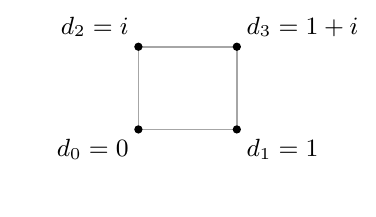
\begin{tikzpicture}[x=1.25cm,y=1.05cm,every node/.style={font=\small}]
  \draw[gray!70,line width=.6pt] (0,0) rectangle (1,1);
  \fill (0,0) circle (1.5pt) node[below left] {$d_0=0$};
  \fill (1,0) circle (1.5pt) node[below right] {$d_1=1$};
  \fill (0,1) circle (1.5pt) node[above left] {$d_2=i$};
  \fill (1,1) circle (1.5pt) node[above right] {$d_3=1+i$};
\end{tikzpicture}
\end{minipage}\hfill
\begin{minipage}[c]{.67\linewidth}
\centering
\begin{tabular}{c@{\qquad}c}
\toprule
$(\sigma_n, \sigma_{n+1})$ & $R_{n+1}-R_n$ \\
\midrule
$01$       & $(1,\ 1,\ 1)$ \\
$12$       & $(-1+i,\ i,\ 1)$ \\
$23$       & $(1,\ -i,\ 1)$ \\
$30$       & $(-1-i,\ -1,\ 1)$ \\
$02,13$    & $(i,\ 1,\ 1)$ \\
$20,31$    & $(-i,\ -1,\ 1)$ \\
\bottomrule
\end{tabular}
\end{minipage}
\caption{Collapse to six steps.}
\label{fig:steps}
\end{figure}

We claim that no three points $R_n$ are collinear.  Suppose otherwise, and
choose $a<b<c$ such that $R_a,R_b,R_c$ are collinear.  Write
$p=b-a$ and $q=c-b$.  Since the last coordinate of $R_n$ is $n$, the affine
parameter is fixed:
\begin{equation}\label{eq:slopes}
 \frac{R_b-R_a}{p}
 =\frac{R_c-R_b}{q}
 =\frac{R_c-R_a}{p+q}.
\end{equation}
In the first complex coordinate this says
\begin{equation}\label{eq:convexity}
 d_{\sigma_b}
 =\frac{q}{p+q}d_{\sigma_a}
  +\frac{p}{p+q}d_{\sigma_c}.
\end{equation}
The four numbers $d_0,d_1,d_2,d_3$ are the vertices of a square.  As each is
an extreme point of their convex hull, the strict convex combination in
\eqref{eq:convexity} forces
\begin{equation}\label{eq:equal-states}
 \sigma_a=\sigma_b=\sigma_c.
\end{equation}

The correction terms $c_{\sigma_n}$ now cancel from the second complex
coordinates in~\eqref{eq:slopes}.  Hence
\begin{equation}\label{eq:gaussian-slopes}
 \frac{z_b-z_a}{p}
 =\frac{z_c-z_b}{q}
 =\frac{z_c-z_a}{p+q}.
\end{equation}
By Lemma~\ref{lem:chords}, for example, we get the square-modulus variations
\[
 \vTwo\!\left(\left|\frac{z_b-z_a}{p}\right|^2\right)
 =\vTwo\bigl(|z_b-z_a|^2\bigr)-2\vTwo(p)=-\vTwo(p).
\]
Thus the three nonzero fractions in~\eqref{eq:gaussian-slopes} have
squared-modulus valuations
\begin{equation}\label{eq:slope-valuations}
 -\vTwo(p),\qquad -\vTwo(q),\qquad -\vTwo(p+q),
\end{equation}
respectively.  Equality in~\eqref{eq:gaussian-slopes} would therefore give
\(
 \vTwo(p)=\vTwo(q)=\vTwo(p+q).
\)
This is impossible: if $p$ and $q$ have the same $2$-adic valuation, then
$p+q$ has a larger one.  Thus no three points of the auxiliary walk $(R_n)$ are collinear..

Finally, list the six possible increments of $R_n$ in Figure~\ref{fig:steps} as
$v_1,\ldots,v_6$.  Starting from $P_0=0$, replace every occurrence of $v_j$
by the standard basis vector ${\bf e}_j\in\N^6$.  The real-linear map
\[
 T:\mathbb R^6\longrightarrow\mathbb C^2\times\mathbb R,
 \qquad T({\bf e}_j)=v_j,
\]
satisfies $T(P_n)=R_n$ for every $n$.  Moreover,
$\sum_{j=1}^6(P_n)_j=n$, so the $P_n$ are distinct.  A collinear triple among
the $P_n$ would map to three distinct collinear points among the $R_n$, which
we have just proved impossible.  This completes the construction.
\end{proof}

\begin{corollary}
The steps of the walk are given by
the unit basis vectors
$({\bf e}_{6,q_i})_{i \geq 0}$,
where $q_i$ is the image under
$\tau$ of the fixed point of the
morphism $\gamma$, defined as follows:
\begin{table}[H]
\centering
\begin{tabular}{c|c|c|c}
$j$ & $\gamma(j)$ & $\tau(j)$ \\
\hline
0 & (0,1) & 0 \\
1 & (2,3) & 1 \\
2 & (4,5) & 2 \\
3 & (0,1) & 3 \\
4 & (6,7) & 4 \\
5 & (8,2) & 2 \\
6 & (4,5) & 0 \\
7 & (3,9) & 5 \\
8 & (10,11) & 1 \\
9 & (6,7) & 5 \\
10 & (10,11) & 4 \\
11 & (9,8) & 3
\end{tabular}
\end{table}
Thus $\tau(\gamma^\omega(0))$ is weakly abelian squarefree.
\end{corollary}




\section{Dimension $3$ and $4$}\label{sec:34}

The constructions here are similar to those of the previous section, except now we use base-$3$ representation and a norm associated with the quadratic form $X^2 - 3Y^2$.

Write $n=\sum_{j\ge0}d_j3^j$ in base $3$ and set
\[
 a_n=(-1)^{d_1+d_3+\cdots},\qquad
 b_n=(-1)^{d_0+d_2+\cdots},\qquad
 R_n=(X_n,Y_n,n),
\]
where $X_n=\sum_{j<n}a_j$ and $Y_n=\sum_{j<n}b_j$. Appending a ternary
digit gives, for $r=0,1,2$,
\begin{equation}\label{eq:rec}
 a_{3n+r}=b_n,\qquad b_{3n+r}=(-1)^r a_n,
\end{equation}
and therefore
\begin{equation}\label{eq:sums}
 X_{3n+r}=3Y_n+r b_n,\qquad
 Y_{3n+r}=X_n+\varepsilon_r a_n,
 \quad(\varepsilon_0,\varepsilon_1,\varepsilon_2)=(0,1,0).
\end{equation}

\begin{lemma}\label{lem:core}
Let $E=\{n\ge0:(a_n,b_n)=(1,1)\}$.  No four points $R_n$ with $n\in E$
are collinear.
\end{lemma}
\begin{proof}
First that $(a_m,b_m)=(a_n,b_n)$ for $m < n$.  Then
\begin{equation}\label{eq:val}
 \vp\!\left((X_n-X_m)^2-3(Y_n-Y_m)^2\right)=\vp(n-m),
\end{equation}
and the expression on the left is nonzero.  To see this, write
$m=3u+r$, $n=3v+s$.  If $r\ne s$, \eqref{eq:rec} gives $b_u=b_v$, so
\[
 X_n-X_m\equiv(s-r)b_u\not\equiv0\pmod3
\]
by \eqref{eq:sums}; both valuations in \eqref{eq:val} are therefore zero.
If $r=s$, then the parent states agree  and
\[
 X_n-X_m=3(Y_v-Y_u),\qquad Y_n-Y_m=X_v-X_u.
\]
Thus the quadratic expression is $-3$ times its parent value and
$n-m=3(v-u)$.  Iteration proves \eqref{eq:val}.

Now suppose $R_{n_0},\ldots,R_{n_3}$, with $n_0<\cdots<n_3$ in $E$, lie
on one line.  There are rational slopes $\alpha,\beta$ such that every
chord has the form
\[
 (X_{n_j}-X_{n_i},Y_{n_j}-Y_{n_i})
   =(n_j-n_i)(\alpha,\beta).
\]
Putting $c=\alpha^2-3\beta^2$, equation \eqref{eq:val} gives
\[
 \vp(n_j-n_i)=\vp(c)+2\vp(n_j-n_i)
\]
for every $i<j$; in particular $c\ne0$.  Hence all six differences have
one common valuation $e= -\vp(c)$.  After division by $3^e$, the four integers
$n_i-n_0$ would be pairwise distinct modulo $3$, impossible.
\end{proof}

Enumerate $E$ as $0=N_0<N_1<\cdots$.  If $n=9q+3u+v$, with $u,v\in\{0,1,2\}$, then by~\eqref{eq:rec} (applied twice)
\[
 (a_n,b_n)=((-1)^ua_q,(-1)^vb_q).
\]
The residues modulo $9$ giving state $(1,1)$ given $(a_q,b_q)$ are respectively
\[
\begin{array}{c|cccc}
(a_q,b_q)&(1,1)&(1,-1)&(-1,1)&(-1,-1)\\ \hline
n-9q&0,2,6,8&1,7&3,5&4
\end{array}.
\]
Notice that $\left(\{(1,1),(1,-1),(-1,1),(-1,-1)\}, \cdot \right)$, where $\cdot$ is the entrywise multiplication forms the Klein-four group, i.e., every element is its inverse and so the table can also be read reversely; starting from $(a_0,b_0)=(1,1)$ one obtains the latter $(a_{n-9q},b_{n-9q})$.

When $q$ is increased by one, a ternary carry changes the parity of exactly
one of the two alternating digit sums (notice that $n=\sum_{j\ge0}d_j3^j  \equiv \sum_{j\ge0} \pmod 2$).
Noticing that the corresponding residue $n-9q$ changes parity as well, reading consecutive entries in the
above table therefore shows that
$N_{k+1}-N_k\in\{2,4,6,8\}.$

In each of the cases, the sum of the $(a_j,b_j)$ depends solely on the difference and one can check the following table,
\begin{equation}\label{eq:return}
\begin{array}{c|cccc}
r=(N_{k+1}-N_k)/2&1&2&3&4\\ \hline
\frac12(R_{N_{k+1}}-R_{N_k})=d_r
 &(1,0,1)&(-1,1,2)&(0,-1,3)&(-2,0,4)
\end{array}.
\end{equation}

For the latter careful check (there are $13$ cases to consider), one sums the corresponding $(a_q,b_q),$ multiplied with the base state (to correspond with $(1,1)$).
For example, if one has $N_i \equiv 5 \pmod 9$ and $N_{i+1} \equiv 4 \pmod 9$,
we have 
\begin{align*}
&(-1,1)\cdot \left( (-1,1)+(1,1)+(1,-1)+(1,1) \right)+ (-1,-1)\cdot \left((1,1)+(1,-1)+(1,1)+(-1,1) \right)\\=&(-1,1)\cdot(2,2)+(-1,-1)\cdot(2,2)=(-4,0),\end{align*}
the latter being two times $(-2,0)$.


\begin{theorem}
There is an infinite standard-basis walk in $\N^4$ with no $4$ collinear
vertices.
\label{thm:d4}
\end{theorem}

\begin{proof}
At the $k$th step use ${\bf e}_{4,r}$, where $r=(N_{k+1}-N_k)/2$.  The linear map
sending ${\bf e}_{4,r}$ to $d_r$ sends the $k$th walk vertex to $R_{N_k}/2$.
Thus four collinear walk vertices would have four collinear images; the
images are distinct because their third coordinates are the distinct
numbers $N_k/2$.  Lemma~\ref{lem:core} gives the contradiction.
\end{proof}

\begin{theorem}\label{thm:d3}
There is an infinite standard-basis walk in $\N^3$ with no seven collinear
vertices.
\end{theorem}
\begin{proof}
The vectors $d_1,d_2,d_3$ in \eqref{eq:return} are independent
(determinant $6$), and $d_1+d_4=d_2+d_3$.  Hence an invertible linear map
may send
\[
 d_1\mapsto {\bf e}_{3,0},\qquad d_2\mapsto {\bf e}_{3,1},\qquad
 d_3\mapsto {\bf e}_{3,0}+{\bf e}_{3,2},
\]
and then necessarily $d_4\mapsto {\bf e}_{3,1}+{\bf e}_{3,2}$.  The images
$S_k$ of $R_{N_k}/2$ therefore form a walk with these four macro-steps,
and Lemma~\ref{lem:core} says that no four $S_k$ are collinear.

Subdivide ${\bf e}_{3,0}+{\bf e}_{3,2}$ as ${\bf e}_{3,2},{\bf e}_{3,0}$ and ${\bf e}_{3,1}+{\bf e}_{3,2}$ as ${\bf e}_{3,2},{\bf e}_{3,1}$.  Every
vertex of the resulting unit-step walk lies in
\[
 \mathcal S\cup(\mathcal S+{\bf e}_{3,2}),\qquad \mathcal S=\{S_k:k\ge0\}.
\]
Each line meets either translate in at most three points, hence contains
at most six vertices altogether.
\end{proof}


\section*{Declaration of AI usage}

Some of the results in this paper were obtained with GPT 6 Astra.

\begin{thebibliography}{99}

%\bibitem{AP16}
%Sergey Avgustinovich and Svetlana Puzynina.
%\newblock Weak abelian periodicity of %infinite words.
%\newblock {\it Theory of Computing Systems} %\textbf{59} (2016), 161--179.

\bibitem{Bro71a}
T. C. Brown.
\newblock Is there a sequence on four symbols in which no two adjacent
segments are permutations of one another?
\newblock {\it Amer. Math. Monthly} {\bf 78} (1971), 886--888.

\bibitem{Bro71b}
T. C. Brown.
\newblock Advanced problem 5811.
\newblock {\it Amer. Math. Monthly} {\bf 78} (1971), 798.

\bibitem{CK26}
Stijn Cambie and Erik Kalviainen.
\newblock An infinite small-step $\Z^3$-walk with no collinear triple.
\newblock Arxiv preprint arXiv:2609.01766 [math.CO],
September 1 2026.  Available at
\url{https://arxiv.org/abs/2609.01766v1}.

\bibitem{FP23}
Gabriele Fici and Svetlana Puzynina.
\newblock Abelian combinatorics on words: a survey.
\newblock {\it Computer Science Review} \textbf{47} (2023), article~100532.

\bibitem{GR79}
Joseph L.~Gerver and L.~Thomas Ramsey.
\newblock On certain sequences of lattice points.
\newblock {\it Pacific Journal of Mathematics} \textbf{83} (1979), 357--363.

\bibitem{Ko26a}
Samuel Korsky.
\newblock North-east lattice paths with few collinear vertices.
\newblock Arxiv preprint arXiv:2607.02832 [math.CO], July 2 2026.
\newblock Available at \url{https://arxiv.org/abs/2607.02832}.

\bibitem{Ko26b}
Samuel Korsky.
\newblock Long lattice paths with no three collinear vertices.
\newblock Arxiv preprint arXiv:2608.07906 [math.CO], August 8 2026.
\newblock Available at \url{https://arxiv.org/abs/2608.07906}.

\bibitem{Lid24}
Thomas F.~Lidbetter.
\newblock Improved bound for the Gerver--Ramsey collinearity problem.
\newblock {\it Discrete Mathematics} \textbf{347} (2024), article~113718.

\bibitem{Mo72}
P. L. Montgomery. 
\newblock Solution to Advanced Problem 5811: 
collinear points on a monotonic polygon.
\newblock {\it American Mathematical Monthly} \textbf{79} (1972), 1143--1144.

\bibitem{OEIS}
N. J. A. Sloane et al.
\newblock The On-Line Encyclopedia of Integer Sequences.
\newblock Electronic resource, 2026.  Available at
\url{https://oeis.org}.





\end{thebibliography}

\end{document}